\section{Background and Objectives}\label{sec:bg}

% \begin{table*}[]
% \centering
% \resizebox{\textwidth}{!}{

% 	% \begin{tabular}{|l|l|l|l|l|l|l|l|}
% 	% \hline
% 	%  & \textbf{Step Functions} & \textbf{Durable Functions} & \textbf{Beldi} & \textbf{Boki} & \textbf{gg} & \textbf{ExCamera} & \textbf{unum} \\ \hline
% 	% \textit{High-level workflow interface}                        & Y & Y & N & N & Y & Y & Y \\ \hline
% 	% \textit{Do not need supplemental services/ purely serverless} & N & N & Y & N & N & N & Y \\ \hline
% 	% \textit{Strong execution guarantee}                           & Y & Y & Y & Y & N & N & Y \\ \hline
% 	% \end{tabular}

% 	\begin{tabular}{|l|l|l|l|l|l|l|l|l|l|}
% 	\hline
% 	 &
% 	  \textbf{Step Functions} &
% 	  \textbf{Durable Functions} &
% 	  \textbf{Beldi} &
% 	  \textbf{Boki} &
% 	  \textbf{Cloudburst} &
% 	  \textbf{Kappa} &
% 	  \textbf{gg} &
% 	  \textbf{ExCamera} &
% 	  \textbf{unum} \\ \hline
% 	\textit{High-level workflow interface}                        & Y & Y & N & N & Y & Y & Y & Y & Y \\ \hline
% 	\textit{Do not need supplemental services/ purely serverless} & N & N & Y & N & N & N & N & N & Y \\ \hline
% 	\textit{Strong execution guarantee}                           & Y & Y & Y & Y & N & Y & N & N & Y \\ \hline
% 	\end{tabular}
% }
% \caption{Comparison with existing work}
% \label{table:positioning}
% \end{table*}


% Large-scale applications composed of many functions~\cite{excamera, gg-atc,
% deathstar} introduce several new challenges to serverless computing. 

In this section, we describe why it is hard to compose large serverless
workflows, why a purely serverless architecture is interesting and what our
objective are.

\subsection{Evolution of Serverless Workflows}

\begin{figure}[t!]
    \centering
    \scalebox{.4}{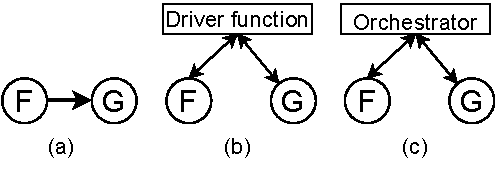
\includegraphics[width=\columnwidth]{figures/ChainExample.pdf}}
    \caption{Chaining two functions with unstructure composition, driver
    functions and orchestrators. In the unstructured composition approach,
	\texttt{F} asynchronously invokes \texttt{G} with \texttt{F}'s result. In
	the driver functions approach, the driver function first synchronously
	invokes \texttt{F} and after \texttt{F} returns, synchronously invokes
	\texttt{G} with \texttt{F}'s result. Even though orchestrators'
	programming interface hides low-level APIs such as \texttt{invoke}, it is
	architecturally similar to driver functions where the orchestrator invokes
	\texttt{F}, waits for \texttt{F} to return and then invokes \texttt{G}
	with \texttt{F}'s result.}
    \label{fig:chain-example}
\end{figure}

\subsubsection{Unstructured composition and driver functions}
While bringing many economical and operational benefits, the original
serverless abstraction is designed around individual functions and only
provides low-level APIs that can be used to compose functions.

There are two primary approaches that early adopters use to build larger
applications. The first approach is sometimes called unstructure
composition~\cite{netherite} where functions trigger each other via
\emph{asynchronous} invocations. The second is often called driver
functions~\cite{beldi} where a single function invokes other functions
\emph{synchronously}. Figure~\ref{fig:chain-example} depicts examples of
chaining functions with the two approaches.

Both approaches have important drawbacks. Unstructure composition scatters
control flow across constituent functions. As the number of functions
increases, development can quickly get unwieldy. Moreover, it does not support
important composition patterns such as fan-in, where we want to invoke a
function to aggregate the results of multiple upstream functions only after
all of them have completed.

Compared with unstructured composition, driver functions concentrate control
flow in a single function and supports aggregation. However, users pay for the
time when driver functions idly wait for callees to return. This causes
\emph{double billing}~\cite{double-billing}. Also, serverless platforms
commonly impose timeouts. A driver function instance has to wait until all
functions in the application are complete, which risks timeouts and limits
application scale.

Moreover, both approaches suffer from weak execution guarantees of the
underlying serverless system. Functions can crash mid-execution due to runtime
or hardware faults which may leads to automatic retries~\cite{}. Even in the
absence of faults, most serverless platforms only ensure at-least-once
execution~\cite{} so a single invocation can trigger multiple, potentially
concurrent, instances.

\subsubsection{Workflow orchestrators}

Recently, workflow orchestrators have emerged to tackle the challenges of
large serverless applications~\cite{excamera, gg-atc, aws-step-functions,
google-cloud-composer, google-workflows, durable-functions}. Orchestrators are
designed as separate hosted services that execute workflow definitions, invoke
constituent functions and manage workflow states. They offer (1). higher-level
programming interfaces that directly express function interactions and hide
low-level APIs, (2). a rich set of composition primitives, including
branching, chaining, fan-out and fan-in, (3). exactly-once semantics for
workflow execution, and (4). long or no runtime limits.

Unfortunately, there are several important drawbacks of the orchestrator
design that compromise key benefits of the serverless abstraction: (1).
End-to-end performance now also depends on the orchestrator service that is
separate from the FaaS engine. A slow orchestrator can become a bottleneck and
nullify the fast autoscale advantage of serverless (2). Architecturally,
orchestrators are similar to driver functions. Service provider cannot
immediately reclaim idle resources from orchestrators which limits
multiplexing and reduces utilization. (3). As a result of (2), service
providers pass the costs of the lost efficiency to users by employing
separately-designed pricing schemes that are coarse-grained and not
pay-for-what-you-use, essentially ``double-charging'' for idle orchestrator
resources that they cannot immediately reclaim. (4). Building and maintaining
a hosted service often requires a dedicated engineering team which is
expensive.

\subsection{Research question and objectives}

In this paper, we examine whether we can have the best of all three worlds. Specifically, we want a system that meets the following objectives:

\paragraph{Higher-level programming interface}

\paragraph{Supports all common interactions}

\paragraph{Exactly-once semantics}

\paragraph{Purely serverless} should not rely on hosted services outside the
serverless abstraction.

\paragraph{Avoids idle waiting} 





% Can we build a workflow system that allows dev to express workflows
% with higher-level interface, supports rich workflow patterns including
% aggregating over multiple functions, while executes purely within the
% serverless abstraction without external services and avoids double billing
% for idle cycles.

% Objective: would such a system be as fast as specially built orchestrators?



%------------------------

% While bringing many economical and operational benefits, the original
% serverless abstraction focuses on building and executing individual functions.
% Support for constructing larger applications that are composed of multiple
% functions is minimum. A key missing feature is an interface to program
% function interactions.

% As a result, early pioneers resort to manually invoking functions and managing
% shared application-wide states~\cite{hello-retail}. For instance, to chain two
% functions, say \texttt{F} and \texttt{G}, \texttt{F} needs to explicitly
% invoke \texttt{G} with \texttt{F}'s result in the source code. Invocations are
% done via asynchronous HTTP requests or storage triggers to avoid waiting. For
% example, Python functions can call Lambda's \texttt{invoke} API via HTTP using
% the AWS \texttt{boto3} sdk. Alternative, developers can configure an S3 bucket
% to generate events on certain storage operations (e.g., writes) that triggers
% \texttt{G}~\cite{aws-s3-event-announce}. Then build \texttt{F} such that it
% writes \texttt{G}'s input data to the pre-configured S3 bucket.

% This approach is often referred to as \emph{unstructured
% composition}~\cite{netherite} because the control flow is scattered across
% functions. Each constituent function contains only a part of the workflow
% logic in its source code.

% There are two main drawbacks of unstructured composition. First, developing
% and maintaining can quickly become unwieldy as the number of functions
% increases. Second, because the invoke API only passes the caller's data, it is
% difficult to support an important composition pattern--fan-in, where we want
% to invoke a function to aggregate the results of multiple upstream functions
% only after all of them have completed.



% Group driver functions and workflow systesm into orchestrators.

% Serverless workflow systems have emerged to solve these
% challenges~\cite{aws-step-functions, google-cloud-composer, google-workflows,
% durable-functions}.




% No higher-level interface to express function interactions. To chain two
% functions, say \texttt{F} and \texttt{G}, \texttt{F} needs to explicitly invoke
% \texttt{G} in its code (for example, Python Lambda functions can invoke other
% functions via Lambda's \texttt{invoke} API with AWS \texttt{boto3} sdk).

% Application states shared across functions have to be manually managed.



% Can we build a system that executes workflows written in with a higher-level
% interface but without a centralized orchestrator service that the platform has
% to host? 

%------------------------

% In the case of orchestrators/coordinators, functions call back to the
% orchestrator when complete and the orchestrator decides what to do next: which
% downstream function to invoke:

% mu: "mu uses a long-lived coordinator that commands and controls a fleet of
% workers."

% gg: "The main entry-point for executing a thunk is the coordinator program....
% Upon start, this program [the coordinator] materializes the target thunk's
% dependency graph... Then, the thunks that are ready to execute are passed to
% execution engines. ... When the execution of a thunk is done, the progra      m [the
% coordinator] updates the graph by replacing the references to the just-forced
% thunk ... The thunks that become ready to execute are placed on a queue and
% passed to the execution engines when their capacity permits."

% Step Functions: TBA


% unum's different: orchestration logic is distributed to each function. When a
% function complete, instead of calling back to a long-lived coordinator, the
% unum runtime on the Lambda decides what to do next. This design eliminates the
% need for a separate long-running service that executes workflows. Saves a
% communication trip back to the orchestrator.



% ----

% ExCamera or mu:

% all workers in mu use the same generic Lambda function that is capable of
% executing the work of any thread in the computation. (change the programming
% interface: developers not writing individual functions anymore. :"To design a
% computation, a user specifies each worker’s sequence of RPC re- quests and
% responses in the form of a finite-state machine (FSM), which the coordinator
% executes.")

% mu uses a long-lived coordinator that commands and controls a fleet of
% workers. The coordinator steps workers through their tasks by issuing RPC
% requests and processing responses. As examples, the coordinator can instruct
% the worker to re- trieve from or upload to AWS S3; establish connections to
% other workers via a rendezvous server; send data to workers over such
% connections; or run an executable.

% Do the output of one worker go through the coordinator to be sent to and
% consumed by another worker? No, there's a separate rendezvous server for
% worker communication. Like the coordinator, the rendezvous server is long
% lived. mu’s rendezvous is a simple relay server that stores messages from
% workers and forwards them to their destination.


% gg's Restrictions on user code: "gg thunks are designed to be deterministic."
% "it is not allowed to use the network or access unlisted objects or files." So
% functions are basically pure so that gg doesn't need to reason about
% exactly-once semantics.


% "In a long chain
% of rebasing, later threads spend much of their time waiting
% on predecessors (Figure 4). A more-sophisticated launch-
% ing strategy could save money, without compromising
% completion time, by delaying launching these threads."

% [This is another point about many of these frameworks, (I think cloudburst has
% this problem as well) that they need to launch custom-built containers *ahead
% of time*, not on-demand, not event-driven. Double billing becomes an issue.
% Utilization becomes an issue.]

% --- 
% Beldi and Boki.

% --- 
% Cloudburst

% ---
